O Software tem duas partes integrantes e plugáveis, o \textit{back-end} e o \textit{front-end}. Ambas as partes podem funcionar separadamente, exercendo seus papéis, ou seja, pode ser conectado outro \textit{front-end} ao \textit{back-end} existente, e vice versa. Desde que siga a arquitetura planejada.

\par O \textit{back-end} pode servir várias instâncias de \textit{fron-end}, estando nos mesmos servidores ou não. Isso tem a idéia de containers, é altamente recomendado instalá-lo em um servidor com estrutura \textit{cloud}, o qual seus recursos de hardware e conexão crescem de acordo com a demanda.

\par É válido ressaltar que podemos separar cada parte do Software em containers, sendo o BD um container, o \textit{back-end} outro, por último, o \textit{fron-end}. Podem ficar em servidores separados (recomendado) ou no mesmo servidor (não é recomendado). Conforme a Figura \ref{fig:arc}.

\begin{figure}[!ht]
  \centering
      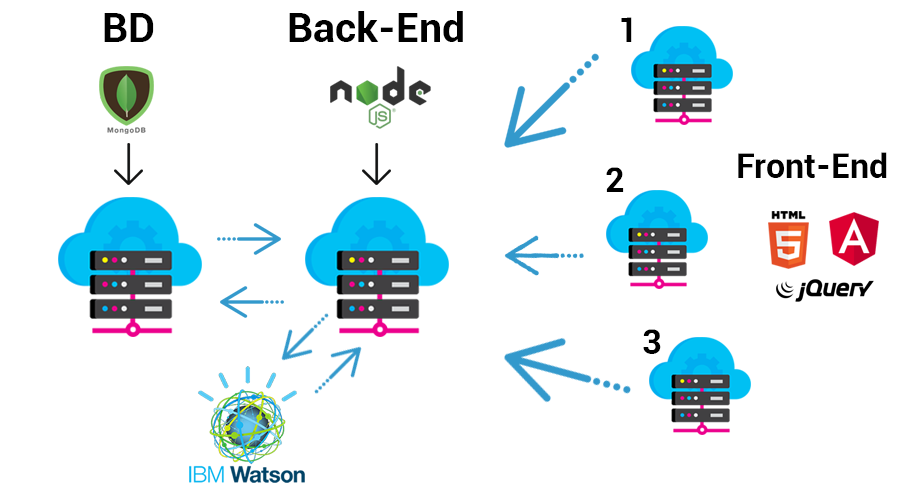
\includegraphics[width=0.55\textwidth]{arc}
  \caption{Arquitetura do Software}
  \label{fig:arc}
\end{figure}